\chapter{Vulnerabilidades}

\section{Introdução}

A OWASP é uma organização sem fins lucrativos que por projetos open-source aspira auxiliar no desenvolvimento de aplicações e ambientes mais seguros. Dentre seus projetos existe a OWASP TOP:10 focado em informar aos profissionais de segurança e demais pessoas interessadas o estado atual da segurança mundial, quais tipos de vulnerabilidades tem sido mais exploradas e com isso chamar atenção para as falhas mais comumente exploradas por invasores, mostrando assim aspectos novos a serem observados com mais atenção nas aplicações. É importante frisar que vários tipos de vulnerabilidades são difíceis de serem quantificadas e monitoradas, por isso a OWASP não se baseia apenas em números de detecções, mas também no estado da arte, publicações e estudo de vulnerabilidades atuais \cite{url:OWASP}.

No ano de 2021 a OWASP TOP:10 publicou um novo informativo, classificando distintamente os tipos de vulnerabilidades antes previstos, criando categorias e alterando também o ranking de cada tópico. Neste ano os tópicos se baseiam muito na adequação as leis que envolvem a proteção de dados dos usuários. Na Figura 3 são apresentados os 10 maiores riscos do ano de 2021 segundo a OWASP.

\begin{figure}[!htb]
     \centering
     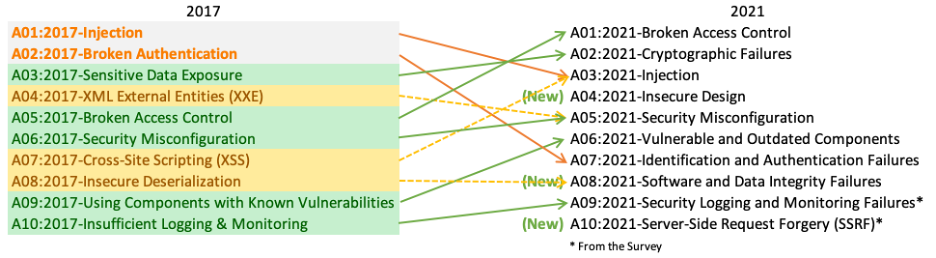
\includegraphics[width=15cm]{mapping.png}
     \caption{Top 10 Web Application Security Risks~\cite{url:OWASP}}
     \label{Label de referência para a imagem}
\end{figure}

% Vulnerabilidades 0day

\section{Broken Access Control}

Broken Access Control é um tipo de vulnerabilidade caracterizada pelo acesso a um ativo indevidamente por um usuário, sistema ou dispositivo não autorizado \cite{hassan2018quantitative}. Em sistemas as permissões de acesso deveriam ser bem definidas. Um sistema de hotelaria, por exemplo, não deveria permitir que um usuário autenticado como um comprador crie anúncios de quartos de Hotel através de um perfil administrativo. Na máquina Mutillidae II \cite{Jeremy2022} existe um exemplo de Broken Access Control, causada por cada usuário ter um \textit{uid} fixo e ordenado crescentemente. Para explorar a falha basta inserir credenciais válidas de qualquer usuário e alterar o \textit{uid} enviado na requisição em um valor de perfil com acessos administrativos.

\section{Cryptographic Failures}

Cryptographic Failures são as vulnerabilidades que expõem dados sensíveis de uma aplicação por conta de uma criptografia fraca ou inexistente \cite{nagoriquantum}. Os dados podem ir desde informações médicas até senhas ou números de cartão de crédito. Nas aplicações modernas os dados passam por manipulações de dados em repouso e em trânsito, tornando ainda mais necessário um controle rígido de criptografia para que essas vulnerabilidades sejam dificilmente aproveitadas. Este tipo de vulnerabilidade estava em terceiro lugar no ano de 2017, mas subiu para segundo lugar no ano de 2021 \cite{url:OWASP}, pois problemas de segurança causados por senhas \textit{hard-coded} tem se tornado muito comuns.

\section{Injection}

Injection é a classe de vulnerabilidades que engloba as falhas que ocorrem no momento que um dado é injetado em uma aplicação e consegue com isso alterar o comportamento planejado da aplicação, tornando, por exemplo, uma simples \textit{string} que serviriam como nome em um código malicioso executável \cite{9319139}. Essas falhas geralmente ocorrem por uma falta de validação das entradas ou uma neutralização imprópria das entradas das aplicações. Como exemplo de Injection temos um caso de SQL Injection, onde se a aplicação tiver dentro de seu código uma execução semelhante a "query = 'SELECT * FROM users WHERE id=' + getParamer("id") + ';'" seria possível dar como id o valor "' or 1=1'" e alterar o sentido original da query já que ela foi projetada para retornar os usuários onde o \textit{id} é igual ao informado, mas com esta injeção toda a tabela é retornada como resposta.

\section{Insecure Design}

Insecure Design é a classe de vulnerabilidades existentes quando um projeto possui problemas de segurança de forma que mesmo que as melhores práticas de desenvolvimento sejam utilizadas o sistema ainda continuará a ser inseguro. Então a causa da falha já faz parte do design escolhido para o projeto que podem levar a, por exemplo, vazamento de informações da aplicação \cite{9935837}. Uma das vulnerabilidades da classe é justamente a "CWE-209 Geração de mensagem de erro contendo informações confidenciais", mas erros como armazenamento desprotegido de credenciais ou violação de limite de confiança também vão ser vulnerabilidades desta classe.

\section{Security Misconfiguration}

Security Misconfiguration em resumo são as falhas de segurança motivadas por falta de configuração ou configuração padrão em aplicações e/ou serviços \cite{6045929}. Quando um banco de dados é configurado com valores padrão e executado em porta padrão, ele carrega inúmeros problemas e falhas de segurança. Falhas que podem ser facilmente encontradas por códigos maliciosas que procuram automaticamente serviços executando em determinadas portas. Nas Security Miscunfigurations também estão faltas por falta de configurações de header.

\section{Vulnerable and Outdated Components}

Vulnerable and Outdated Components é a classe que engloba as vulnerabilidades que envolvem as falhas por conta de componentes de software datados ou que possuem falhas conhecidas que são adicionados ao serviço em questão \cite{galvao2022analysis}. Durante o desenvolvimento de novos serviços é difícil criar tudo do zero, sendo comum, que sejam utilizados componentes prontos de terceiro, o problema é que quando um componente com falha é adicionado em uma aplicação, essa aplicação obviamente herda a vulnerabilidade que pode ou não ter algum peso no contexto da aplicação. 

\section{Identification and Authentication Failures}

Identification and Authentication Failures é a classe que aloca as falhas que envolvem controle de autenticação, como quebra em gerenciamento de sessão de usuários por má implementação do serviço \cite{authentication}. Essas falhas podem ter origens como: não tratamento para força bruta, permissão de senhas fracas, permissão de usuários default, processos ineficiente de recuperação de credenciais, e reutilização de identificadores de sessão. Muitas ferramentas são desenvolvidas para automatizar a exploração dessas vulnerabilidades, no caso de não tratamento de força bruta é possível explorar com ataques de dicionário.

\section{Software and Data Integrity Failures}

Software and Data Integrity Failures é a classe de vulnerabilidades que se aproveitam da falta de confirmação de integridade do software e de dados \cite{integrity}. Pode ocorrer, por exemplo, quando uma aplicação usa fontes externas não confiáveis, quando não existe um pipeline seguro no CI/CD, quando um invasor pode obter acesso a dados e/ou estruturas que possam ser vistas e alteradas. 

\section{Security Logging and Monitoring Failures}

O item Security Logging and Monitoring Failures da OWASP TOP Ten vai além de apenas classificar falhas, mas visa abordar os tópicos de resposta e monitoriamento dos ataques realizados em um ambiente \cite{logging}. Esta etapa se mistura com vários itens do OWASP TOP Ten, uma vez que para um correto monitoramento é necessário ter os logs armazenados seguramente, portanto um design correto para isso é necessário assim como confirmar a integralidade dos logs para se necessário usar os mesmos como provas. Dentro dessa classe de falhas é importante entender que além de logs insuficientes nas aplicações, logs com dados sensíveis também podem gerar problemas de segurança e logs com dados demais podem dificultar o monitoramento.

\section{Server-Side Request Forgery}

Server-Side Request Forgery como o nome diz, é uma vulnerabilidade causada pela falsificação de uma requisição do lado do servidor e ela acontece quando o servidor recupera o conteúdo de uma requisição, mas por não validar o URL acaba não garantindo que a requisição chegue ao destino esperado, esta falha tem um CWE mapeada que é a CWE-918 \cite{jabiyev2021preventing}. Esta vulnerabilidade consegue enviar as requisições a destinatários mesmo quando protegidos por firewall, VPN ou outro ACL.